%
% problemstellung.tex -- Beispiel-File für die Beschreibung des Problems
%
% (c) 2020 Prof Dr Andreas Müller, Hochschule Rapperswil
%
\section{Iteration der logistischen Gleichung
\label{logistic:section:problemstellung}}
\rhead{Iteration der logistischen Gleichung}

Auf der Abbildung \ref{fig:pop_logistic} ist ersichtlich, 
dass $x_n$ beim Iterieren der logistische Gleichung
für verschiedene Werte von $\lambda$ auf verschiedene
Werte konvergiert. 

\begin{figure}
    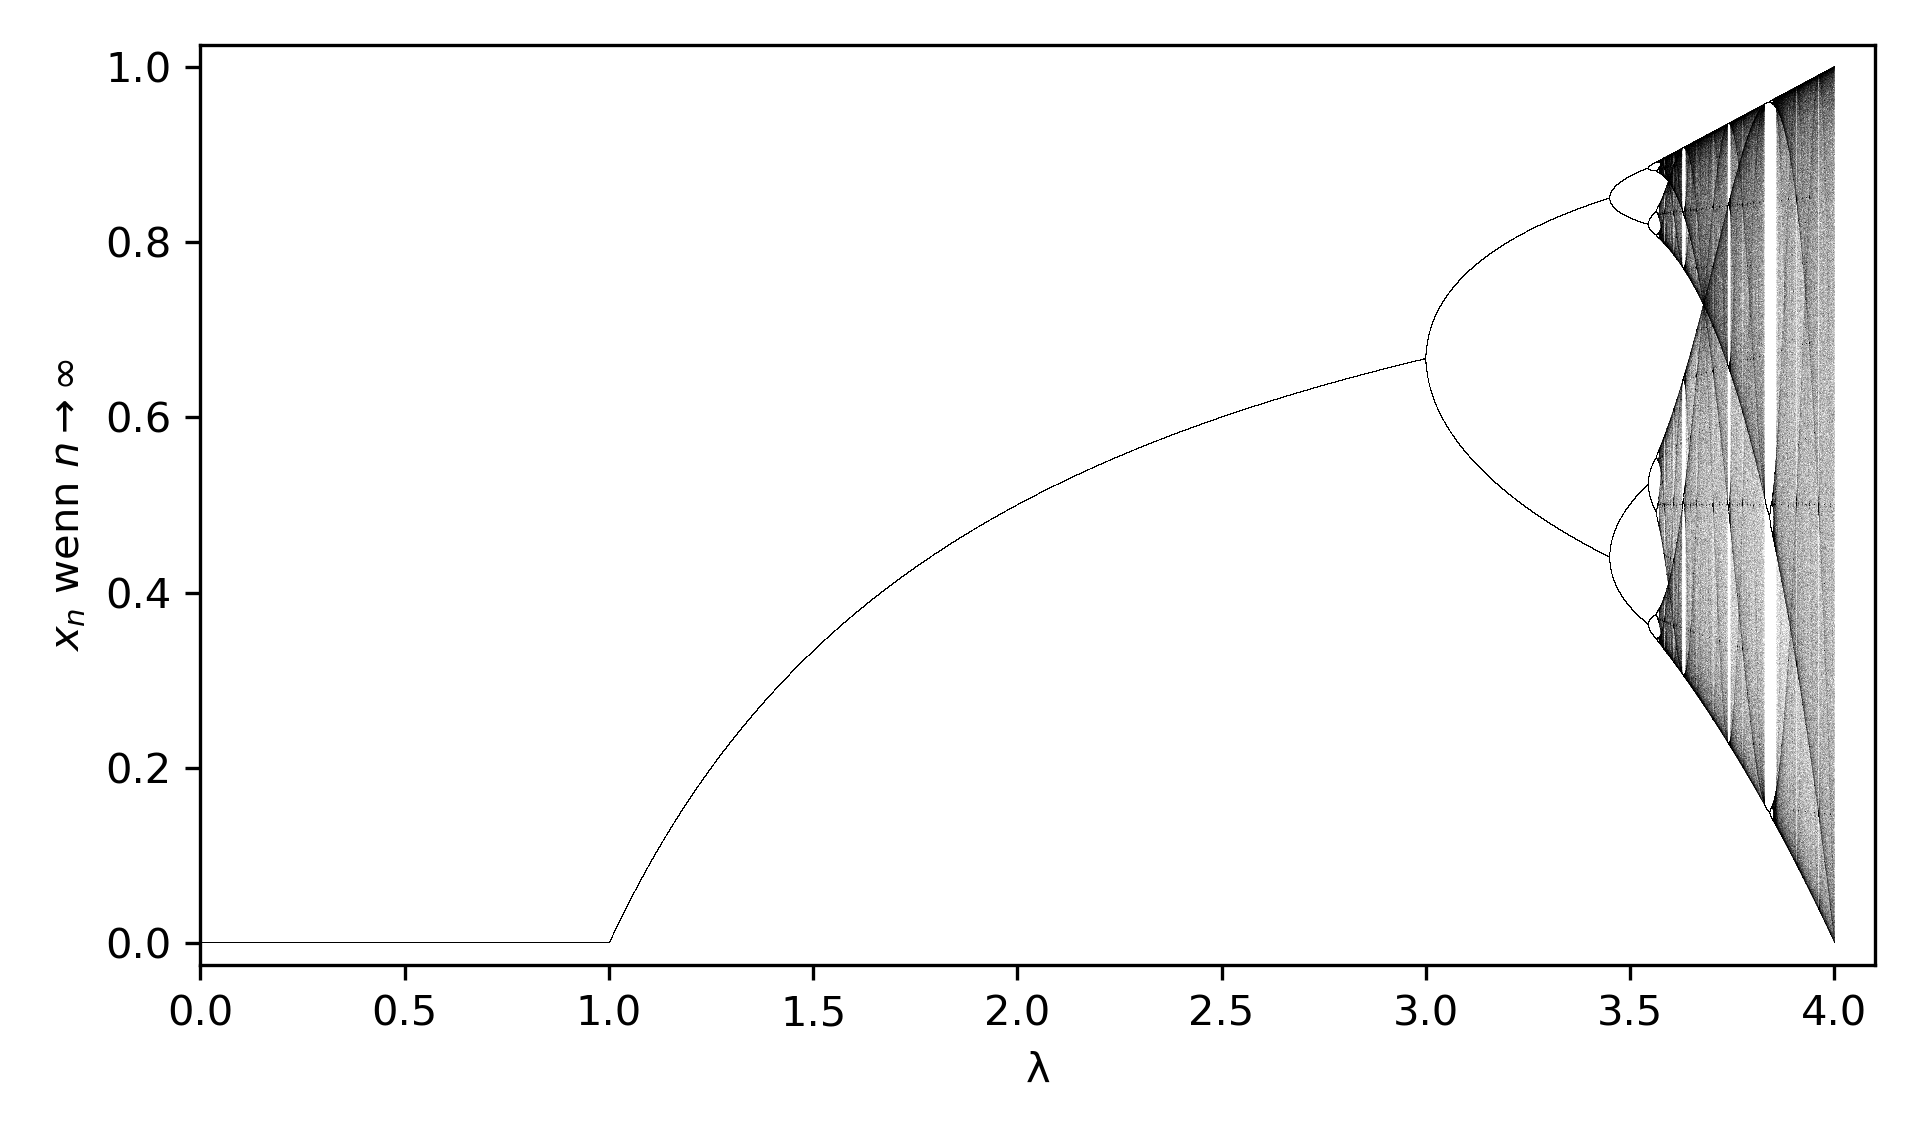
\includegraphics[width=\linewidth]{papers/logistic/figures/map.png}
    \caption{Bifurkationsdiagramm der logistischen Gleichung}
    \label{fig:map_1}
\end{figure}

Abbildung \ref{fig:map_1} zeigt nun einen Plot, 
auf dem die horizontale Achse die verschiedenen Werte
von $\lambda$ annimmt und die vertikale Achse anzeigt,
auf welchem Wert $x_n$ konvergiert, wenn $n$ gegen
unendlich läuft. Darauf werden einige Eigenschafen 
von der Iteration der logistischen Gleichung ersichtlich:

\begin{itemize}
    \item 
    für $0 \le \lambda \le 1$ konvergiert $x$ gegen 0
    \item 
    für $1 \le \lambda \le 3$ konvergiert $x$ gegen einen fixen Wert
    \item 
    für $\lambda > 3$ scheint $x$ nicht mehr gegen einen fixen Wert zu konvergieren.
    Stattdessen gibt es diese Verzweigungen, 
    die darauf hindeuten, 
    dass $x$ zuerst bis $\lambda \approx 3.4$ auf zwei Werte konvergiert, 
    dann bis $\lambda \approx 3.6$ auf vier Werte, dann 8, 16, usw. 
\end{itemize}

\begin{figure}
    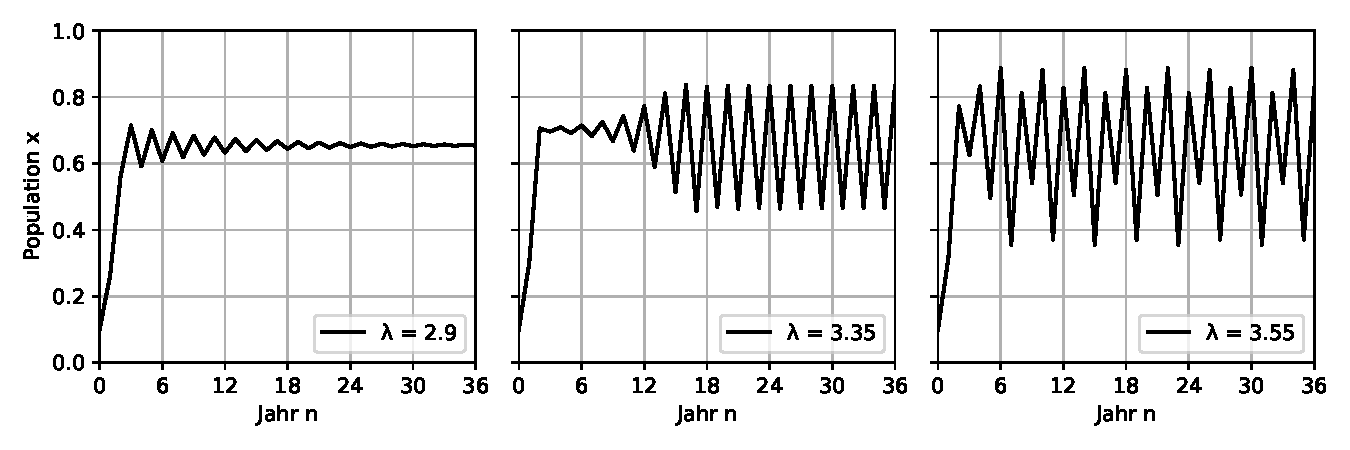
\includegraphics[width=\linewidth]{papers/logistic/figures/pop_logistic_2.pdf}
    \caption{Iteration der logistischen Gleichung}
    \label{fig:pop_logistic_2}
\end{figure}

Das Verhalten von $\lambda > 3$ wird auch in Abbildung 
\ref{fig:pop_logistic_2} ersichtlich,
wenn man die Werte der einzelnen Iteration plottet.
Im ersten Plot sieht man, dass $x$ zuerst oszilliert,
aber schliesslich auf einen fixen Wert konvergiert.
Auf dem zweiten Plot mit $\lambda = 3.35$ scheint $x$ 
für immer zwischen zwei Werten zu oszillieren und beim
dritten Plot sogar zwischen vier Werten. 
Dieses Oszillieren zeigt sich in Abbildung \ref{fig:map_1}
durch die Verzweigungen oder auch "Bifurkationen". 
Darum wird es auch "Bifurkationsdiagramm" genannt. 

